\documentclass[a4paper,12pt]{article}

\usepackage[slovak]{babel}
\usepackage[left=1.5cm,text={18cm, 25cm},top=2cm]{geometry}
\usepackage[utf8]{inputenc}
\usepackage{times}
\usepackage{amsthm}
\usepackage{amsmath,amsfonts,amssymb}
\usepackage{graphicx}
\usepackage{rotating}
\usepackage{listings}
\usepackage{xcolor}
\usepackage{microtype}
\usepackage{textcomp}
\usepackage{caption}
\usepackage{relsize}
%\usepackage{subcaption}
\usepackage{subfig}
\usepackage{placeins}

\definecolor{codegreen}{rgb}{0,0.6,0}
\definecolor{codegray}{rgb}{0.5,0.5,0.5}
\definecolor{codepurple}{rgb}{0.58,0,0.82}
\definecolor{backcolour}{rgb}{0.95,0.95,0.92}

\lstdefinestyle{mystyle}{
    backgroundcolor=\color{backcolour},   
    commentstyle=\color{codegreen},
    keywordstyle=\color{magenta},
    numberstyle=\tiny\color{codegray},
    stringstyle=\color{codepurple},
    basicstyle=\ttfamily\footnotesize,
    breakatwhitespace=false,         
    breaklines=true,                 
    captionpos=b,                    
    keepspaces=true,                 
    numbers=left,                    
    numbersep=5pt,                  
    showspaces=false,                
    showstringspaces=false,
    showtabs=false,                  
    tabsize=2,
    extendedchars=false,
    escapeinside={\%*}{*)},
    inputencoding=utf8
}
\lstset{style=mystyle}

\author{Jakub Mĺkvy (xmlkvy00)\\Adam Múdry (xmudry01)}
\date{\today}
\title{\Large\bf Projekt -- IMS 2020/2021}

\begin{document}
\begin{titlepage}
	\begin{center}
	    \vspace*{+3cm}
		\Huge
		\textsc{Fakulta informačních technologií\\
		\huge Vysoké učení technické v~Brně}\\
		\vspace{\stretch{0.382}}    
	    {\LARGE{Dokumentácia\\Projekt č. 11 do predmetu \textit{Modelování a simulace}\\
		 \vspace{4mm}
		 \Huge\textbf{{Modely přírodních a ekologických katastrof\\(Lesné požiare)}}\\
		 \vspace{4mm}
		 2020/2021
		 }}
		 
		\vspace{\stretch{0.618}}
	\end{center}
	{\Large \hfill Jakub Mĺkvy (xmlkvy00)\\
	\today \hfill Adam Múdry (xmudry01)}
	
	\thispagestyle{empty}
    \setcounter{page}{0}
\end{titlepage}

\newpage

\tableofcontents

\newpage
\section{Spustenie}
Úlohou tohto projektu bolo naprogramovať program (\textit{ims}), ktorý simuluje prírodné a ekologické katastrofy, v našom prípade lesné požiare.
\\
\\
Zoznam odovzdaných súborov: 
\begin{lstlisting}
src/main.cpp src/map.hpp src/cell.hpp src/etc.hpp
Makefile
dokumentacia.pdf
README.md
\end{lstlisting}

\subsection{Preklad}
Program sa prekladá pomocou nástroja {\bf make} spusteného v koreni priečinku:
\begin{lstlisting}
make
\end{lstlisting}
alebo
\begin{lstlisting}
make build
\end{lstlisting}
\leavevmode\\
Pre vytvorenie ladiacej verzie programu použite príkaz:
\begin{lstlisting}
make build-debug
\end{lstlisting}
\leavevmode\\
Makefile spúšťa program \textbf{g++} s nasledujúcimi parametrami:
\begin{lstlisting}
--std=c++17 -Wall -Wpedantic [-O3|-g]
\end{lstlisting}
a linkuje vytvorené objektové súbory na knižnice pomocou:
\begin{lstlisting}
 -lglut -lGLU -lGL
\end{lstlisting}
\leavevmode\\
Vytvára sa spustiteľný súbor {\bf ims} na koreni priečinku.

\subsection{Použitie}
Príkaz na spustenie (GUI verzia):
\begin{lstlisting}
make run ARGS="argumenty"
\end{lstlisting}
alebo priamo cez vygenerovaný spustiteľný súbor:
\begin{lstlisting}
./ims [-h|--help] [-g|--gui] [-l|--log] [-x <x_value>] [-y <y_value>] [-w <N|NW|W|SW|S|SE|E|NE>] [-i|--intensity <i_value>]
\end{lstlisting}
\begin{lstlisting}
%*Príznaky a argumenty*):
    -h, --help                        %*Ukáže pomocnú hlášku*)
    -g, --gui                         %*Spustí aplikáciu v GUI móde*)
    -l, --log                         %*Zapnutie zapisovania do log súboru output.txt*)
    -x <x_value>                      %*Nastavenie začiatočnej X súradnice*)
    -y <y_value>                      %*Nastavenie začiatočnej Y súradnice*)
    -w, --wind <N|NW|W|SW|S|SE|E|NE>  %*Nastavenie smeru vetra*)
    -i, --intensity <i_value>         %*Nastavenie intenzity vetra*)
\end{lstlisting}
Pred použitím programu musí existovať jeho spustiteľný súbor.

Pri spustení programu v móde s grafickým rozhraním (GUI) môžete kliknutím do mapy vytvoriť daľšie ohnisko.

\section{Úvod}

\par\quad Lesný požiar sa v realite šíri a udržuje podľa veľkého množstva faktorov.
Zohľadnenie týchto faktorov vedie k extenzívnym ale presným modelom pre simuláciu.
Jedným z týchto modelov je \textbf{ABBAMPAU model}\cite{simulations}, ktorý zahŕňa faktory
\textit{výška, typ vegetácie, teplota, vlhkosť, typ horenia, dĺžka horenia,
smer vetra, sila vetra, horlavosť}.
Riadi sa štvorcovými bunkami a \textbf{Moorovym algoritmom najbližších susedov}
(algoritmus sa pozerá na štyroch hraničných a štyroch diagonálnych susedov).
\\
\par Ďalší s extenzívnych modelov je \textbf{Rothermelov model} \cite{fireSpread}, ktorý sa sústreďuje na fyzické vlastnosti ohňa
a jeho propagáciu v poveternostných podmienkach. Zohľadňuje aj lietajúce kusy horiaceho materiálu,
ktorý sa rozširuje ohňom, tzv. \textbf(spotting).
\\
\par Tieto modely na svoje spracovanie potrebujú veľké množstvo dát buď o samotnej oblasti, 
alebo typoch paliva na predurčenie správania ohňa.
V našej simulácii sa zaoberáme simplifikovaním pár z týchto faktorov. 
\\
\par Ďalej pri celulárnych automatoch na základe Moorovho algoritmu najbližších susedov,
dochádza k skresleniu bezprostrednej propagácie vďaka svojmu štvorcovému tvaru šírenia. Riešenie tohto problému by mohlo byť využitie 
\textbf{Von Neumanovho algoritmu najbližších susedov} (branie 4-och susedov, ktotrý zdielajú hranu s aktívnou bunkou). Využitie tohto algoritmu by malo
za dôsledok príliš slabej bezprostrednej propagácie horenia. Ďalším riešením by bolo delenie mapy na hexagonálnu mriežku, čo sme ale kompletne vylúčili.
\\
\par Táto simulácia využíva kompromis medzi Moorovym a Von Neumanovym algoritmom, kde rátame aj so susedmi,
s ktorými aktívna buňka zdiela vrchol ale patria do vyššieho rádu.
\\
\par Jedným z hlavných problémov bolo \textbf{minimalizovanie potreby zberu dát} o simulovanej časti mapy, 
tak aby simulácia stále zodpovedala reálnemu požiaru. 
To sme obmedzili na \textbf{hustotu, rýchlosť horenia a šancu vsplanutia pri dvoch distinktívnych typoch 
vegetácie (strom a porast)} kde jedna buňka zodpovedá približne $2,5m^{2}$
ako priemerný zhluk našich dvoch typov vegetácie. 
\\
\par Mapu sme prispôsobili velkosťou nášmu pozorovanému 
prípadu požiaru v článku o smulácii \textbf{požiaru ostrova v Grécku z roku 1990} \cite{CAmodel4FF}
kde postihnutá plocha má $6km^{2}$ a požiar trvá 11 hodín pri tak isto dvoch distinktývnych typov vegetácie a miernom vetre.
\\
\par Výhodou nášho riešenia je, že \textbf{netreba exportovať reálnu oblasť} s mapami typov vegetáncie.
Zhluky a hustotu v zhlukoch, v ktorých sa tieto typy nachádzajú v prírode \textbf{generujeme pomocou pseudonáhodných funkcii}.
\\
\par S kalibráciou horenia nám pomáhal projektant požiarnej bezpečnosti ako naša odborná konzultácia. 

\newpage


\section{Rozbor tématu a použitých metód/technológií}

\subsection{Šírenie ohňa}
Rozdielne stavov šírenia: \\
- šírenie z porastu na porast 
\begin{lstlisting}[language=C++]
newMap[i][j].flammability += std::pow(0.12, distance); 
\end{lstlisting}
- šírenie z porastu na strom 
\begin{lstlisting}[language=C++]
newMap[i][j].flammability += std::pow(0.1, distance); 
\end{lstlisting}
- šírenie zo stromu na strom 
\begin{lstlisting}[language=C++] 
newMap[i][j].flammability += std::pow(0.1, distance); 
\end{lstlisting}
- šírenie zo stromu na porast 
\begin{lstlisting}[language=C++]
newMap[i][j].flammability += std::pow(0.08, distance); 
\end{lstlisting}
- spotting implementovaný ako druhá vzdialenosť šírenia (2. a 3. rád algoritmu najlbližších susedov)

\subsection{Algoritmus najbližších susedov}
Kompromis medzi Von Neumanovym a Moorovym algoritmom. Odvodený vzorec na rátanie pravdepodobnosti vsplanutia pre maximálnu vzdialenosť susedov 2: \quad $\mathlarger{\mathlarger{4x_{0}+16x_{1}^{2}+4x_{2}^{3}}}$
\\
\begin{figure}[htp]
    \centering
    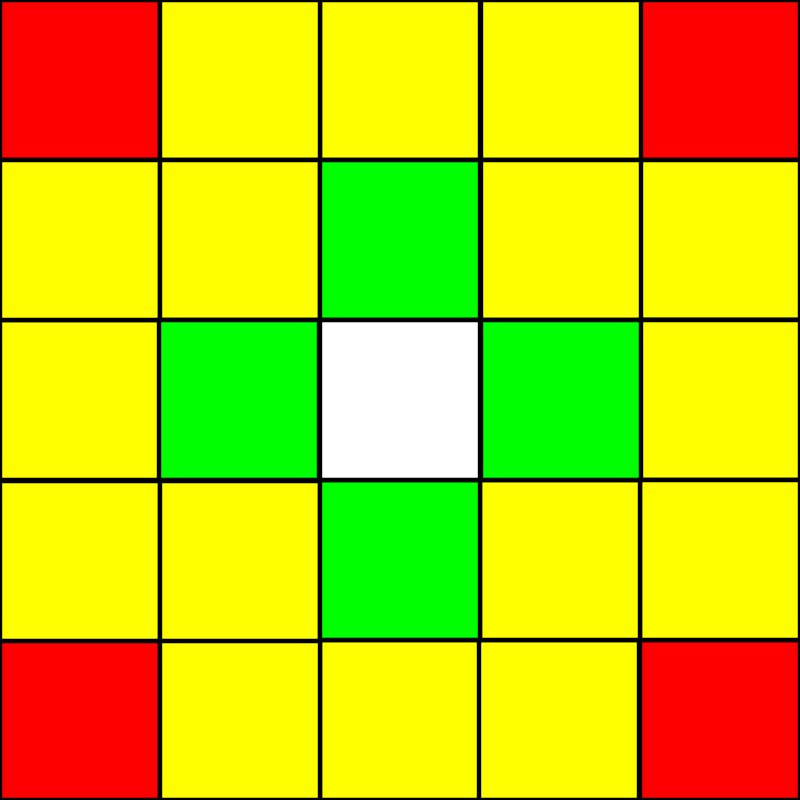
\includegraphics[width=5cm]{neighbor_radius.png}
    \captionsetup{justification=centering,margin=2cm}
    \caption{Zobrazenie rádov buniek ovplivňujúce pravdepodobnosť vsplanutia kde najväčší rád bunke pridáva najmenšiu pravdepodobnosť.\\\textit{Biela} - aktuálna bunka, \textit{zelená} - bunky $(x_{0})$ 1. rádu,\\\textit{žltá} - bunky $(x_{1})$ 2. rádu, \textit{červená} - bunky $(x_{2})$ 3. rádu}
    \label{fig:neighbor_radius}
\end{figure}

\subsection{Vietor}
Napomáha šíreniu ohňa rozširovaním algoritmu najlbližších susedov do danej strany (4 svetové strany a ich kombinácie) o n-tú vzdialenosť, pričom sila vetra je n.

\newpage

\subsection{Generovanie mapy}
Pre generovanie jednotlivých buniek vegetácie používame jednoduchú pseudonáhodnú funkciu: \\
\begin{lstlisting}[language=C++]
float pseudo_rand()
{
  return (float)rand()/13376.9f;  
}
\end{lstlisting}
Vytvarovanie do zhlukov vzniká prehnaním našej pseudonáhodnej funkcie Perlinovým algoritmom hluku \cite{Pnoise}, ktorý nám dám vzor.
Ďalej rozhodujeme či sa bunka nachádza vo vygenerovanom vzore (štruktúra lesa), ak áno tak má šancu byť aktívna na základe faktoru hustoty vegetácie.

\section{Koncepcia}
Model:\cite{konceptModel}
\begin{figure}[htp]
    \centering
    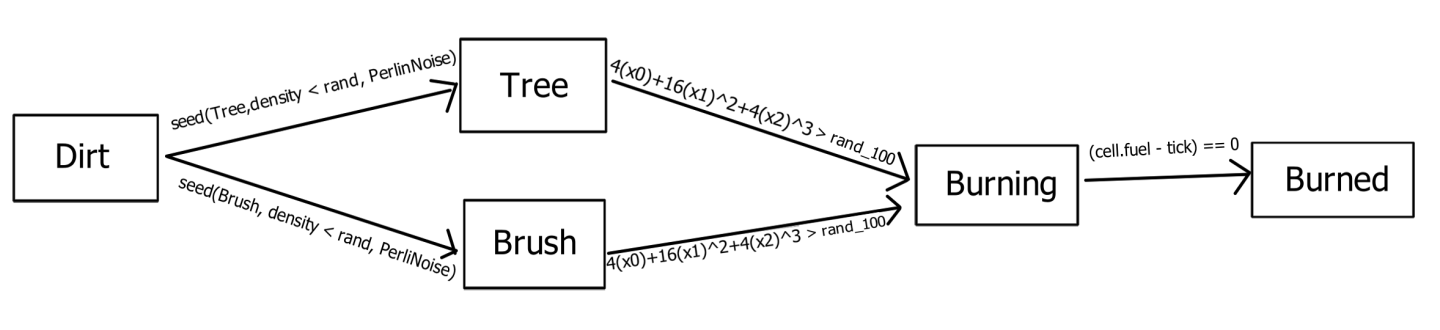
\includegraphics[width=15cm]{koncept.png}
\end{figure}

\newpage
\section{Experimenty}
Experimentovali sme s rôznymi nastaveniami našej simulácie kvôli dosiahnutiu výsledku, ktorý najbliššie simuluje realitu -
menili sme schopnosť rozširovania sa pre oheň, rôzne sily vetra (bezvetire a sily 1 až 3), rôzne začiatočné pozície pre vznik požiaru.
Podľa našeho vzoru \cite{CAmodel4FF} sa nám pri slabých poveternostných podmienkach podarila reprodukcia tvaru aj veľkosti postihnutej oblasti požiarom
aj pri zohladnení minimálneho počtu faktorov.
\\\\
Nižšie uvedené grafy zobrazujú zmenu za čas (v našom prípade tick - 1 kolo simulácie) pre nehoriace bunky, horiace bunky, zhorené bunky
a postihnuté bunky (zhorené + horiace).

\begin{figure}[htp]
    \centering 
    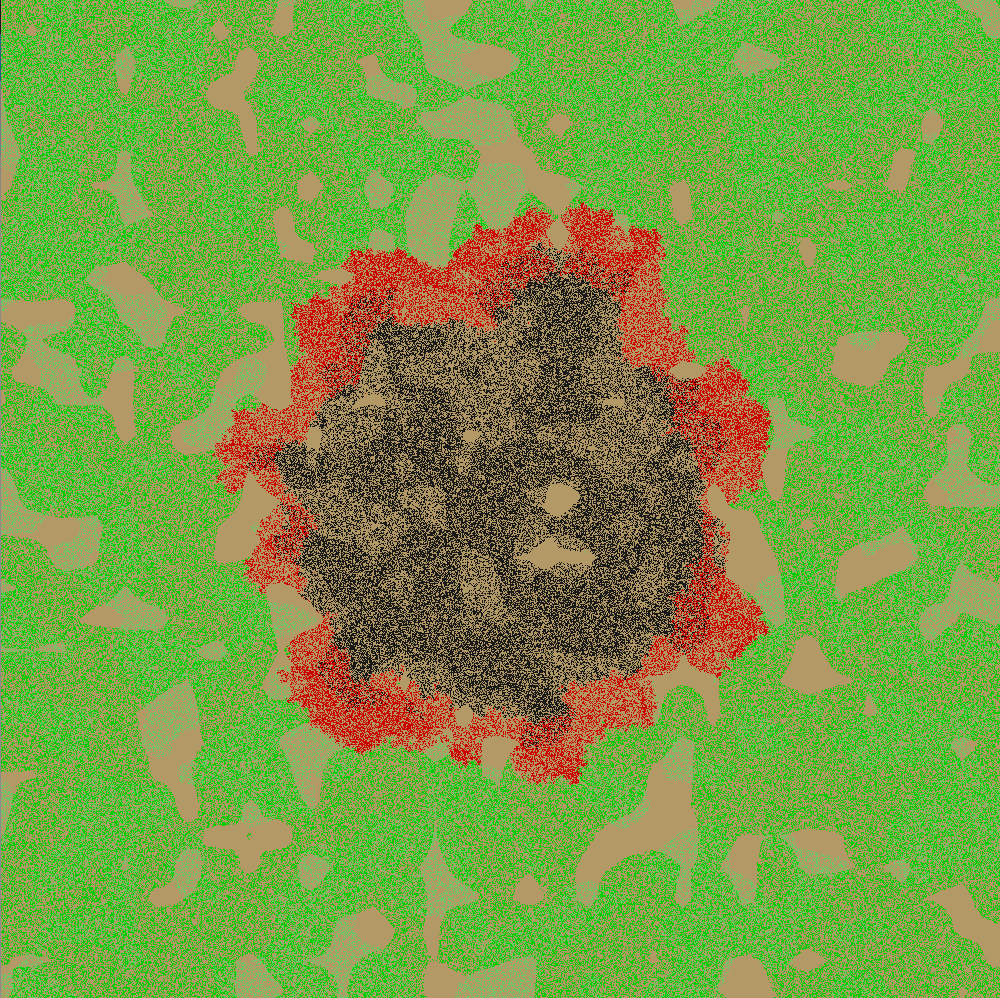
\includegraphics[width=8cm]{none.png}
    \caption{Názorná ukážka simulácie pre bezvetrie so začiatkom požiara na súraidniciach x=500, y=500}
\end{figure}

\begin{figure}[htp]
    \centering
    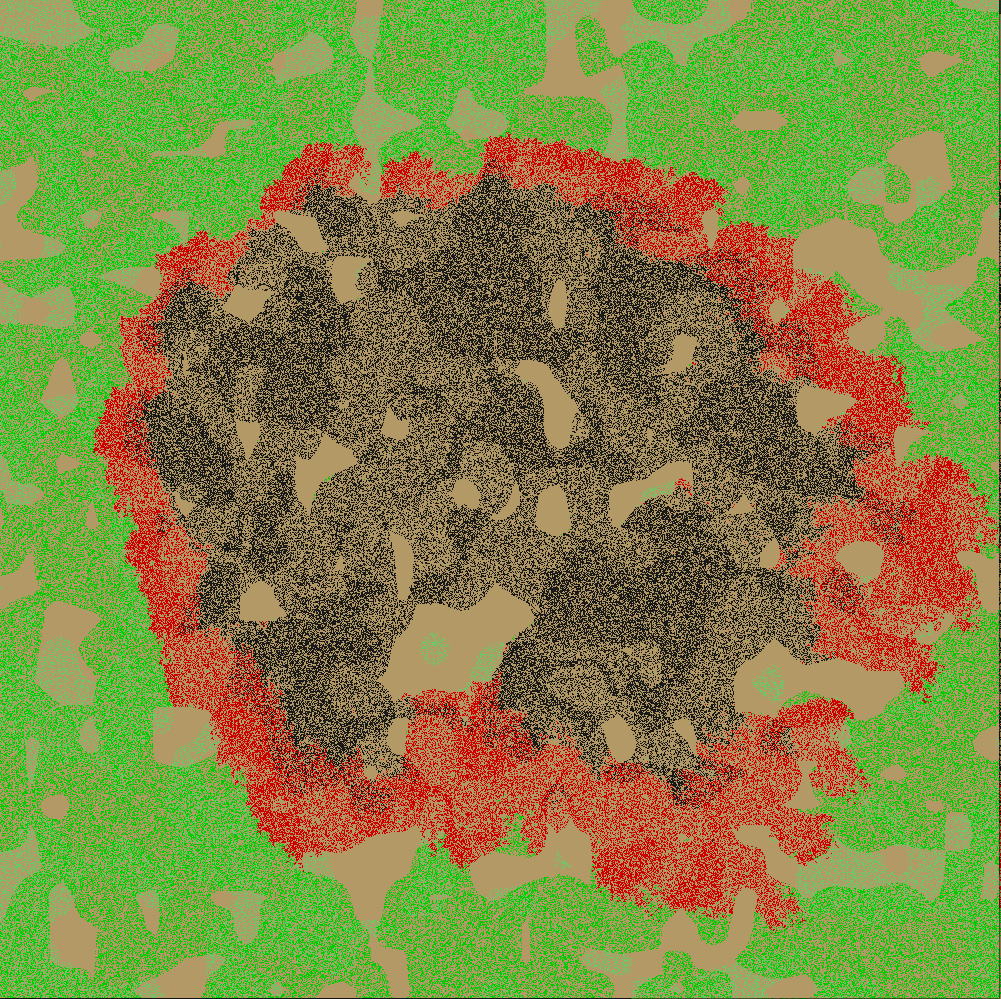
\includegraphics[width=8cm]{se.png}
    \caption{Názorná ukážka simulácie pre vietor fúkajúci na juhovýchod so začiatkom požiara na súraidniciach x=400, y=400}
\end{figure}

\FloatBarrier
\begin{figure}
    \centering
    \subfloat[\centering Bezvetrie]{{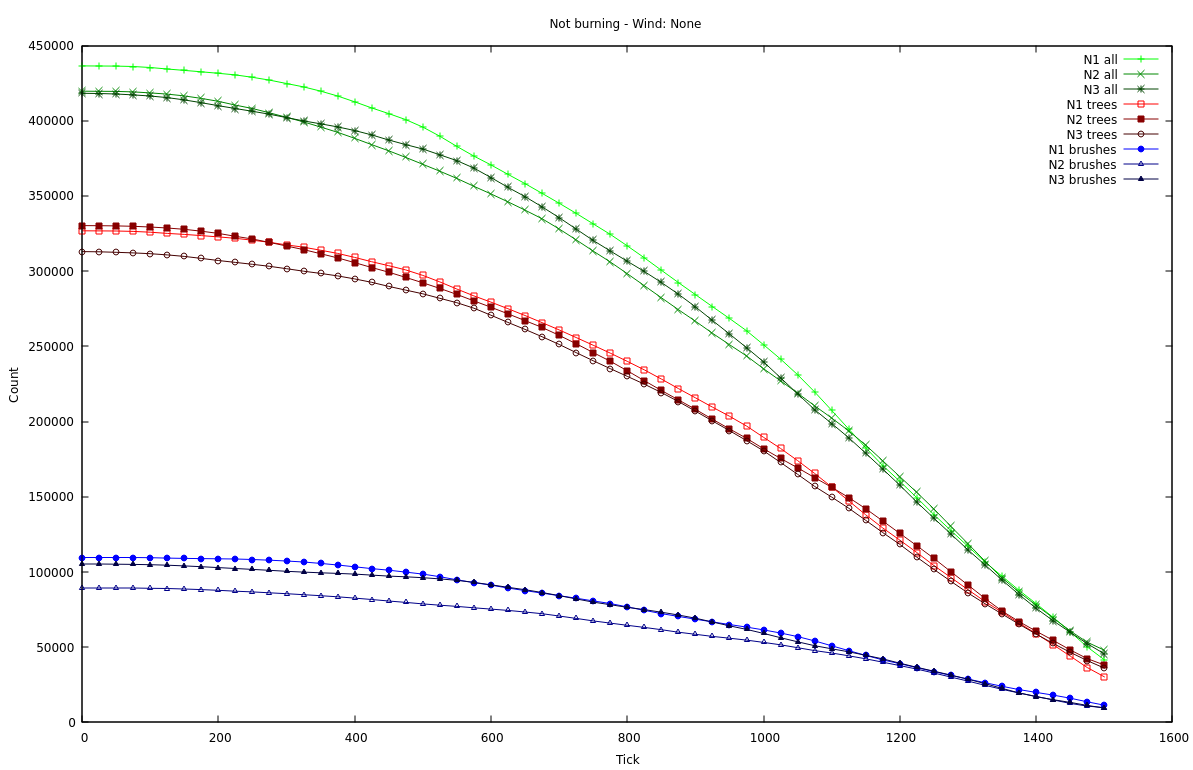
\includegraphics[width=8.2cm]{../output/not_burning/not_burning_none.png} }}
    \qquad
    \subfloat[\centering Slabý vietor]{{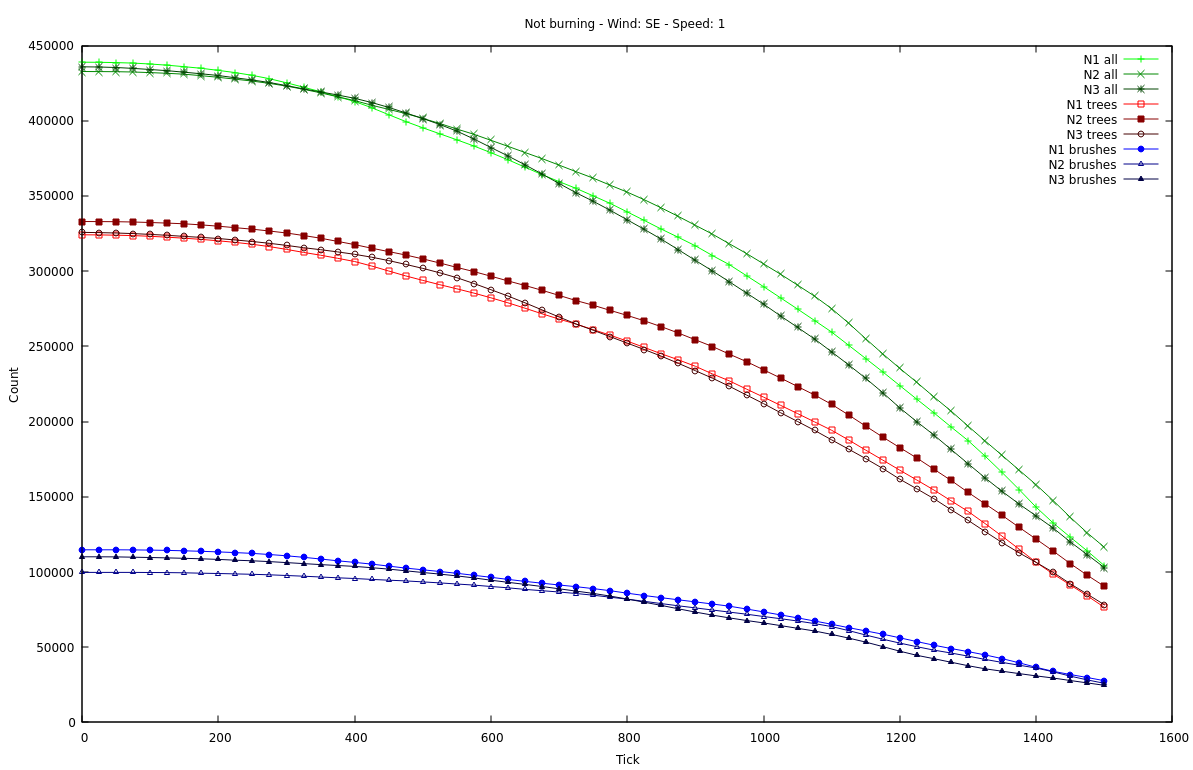
\includegraphics[width=8.2cm]{../output/not_burning/not_burning_se1.png} }}
    \subfloat[\centering Silný vietor]{{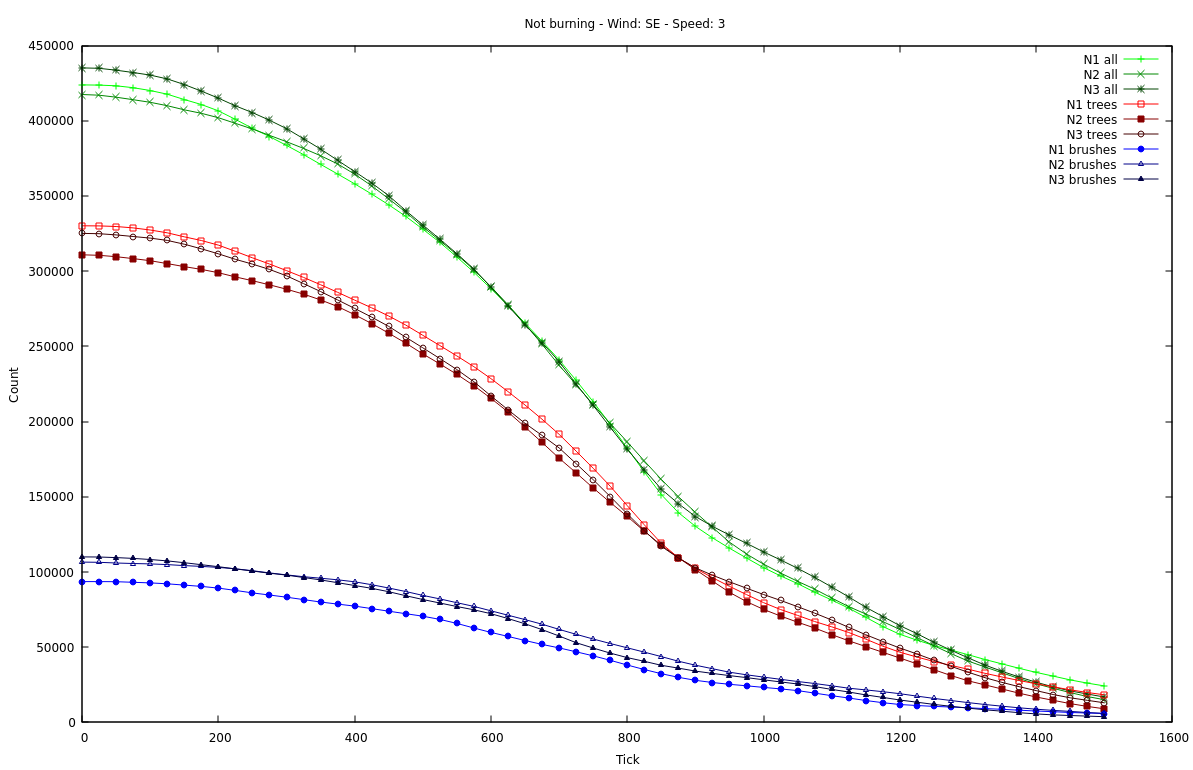
\includegraphics[width=8.2cm]{../output/not_burning/not_burning_se3.png} }}
    \caption{Grafy pre nehoriace bunky pri rôznych poveternostných podmienkach}

    \label{fig:not_burning}
\end{figure}

\FloatBarrier
\begin{figure}
    \centering
    \subfloat[\centering Bezvetrie]{{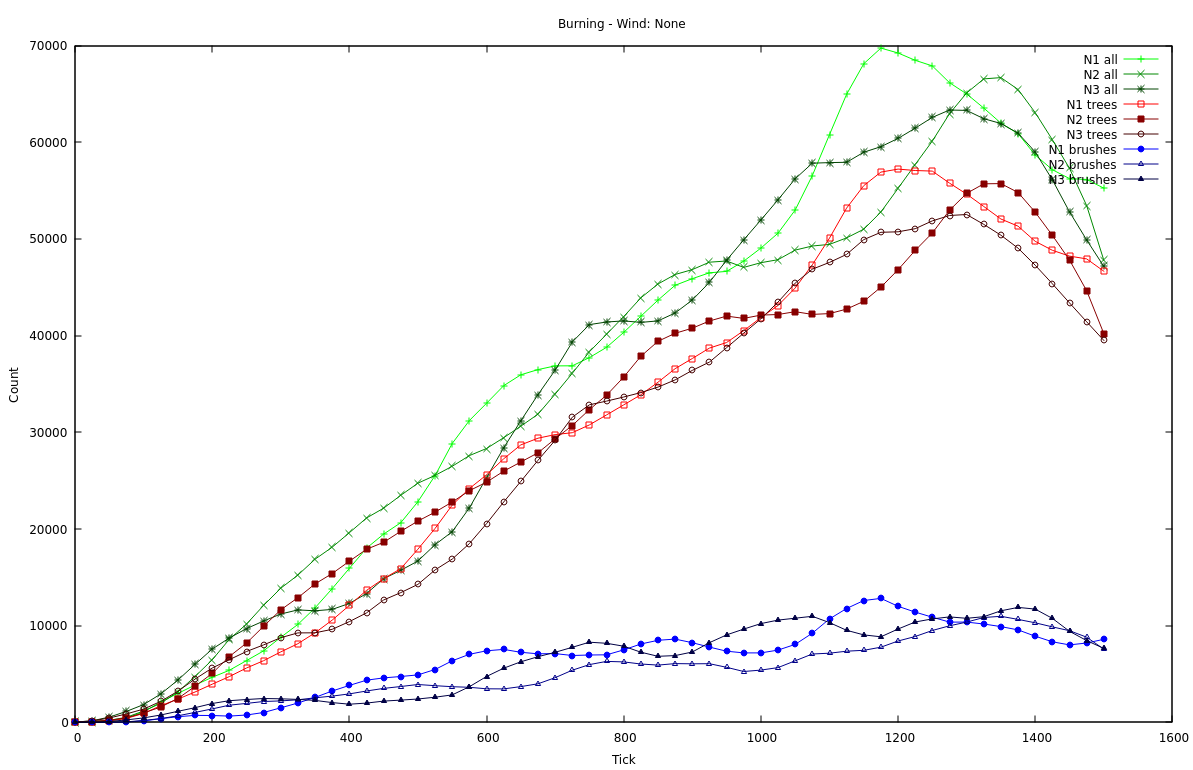
\includegraphics[width=8.2cm]{../output/burning/burning_none.png} }}
    \qquad
    \subfloat[\centering Slabý vietor]{{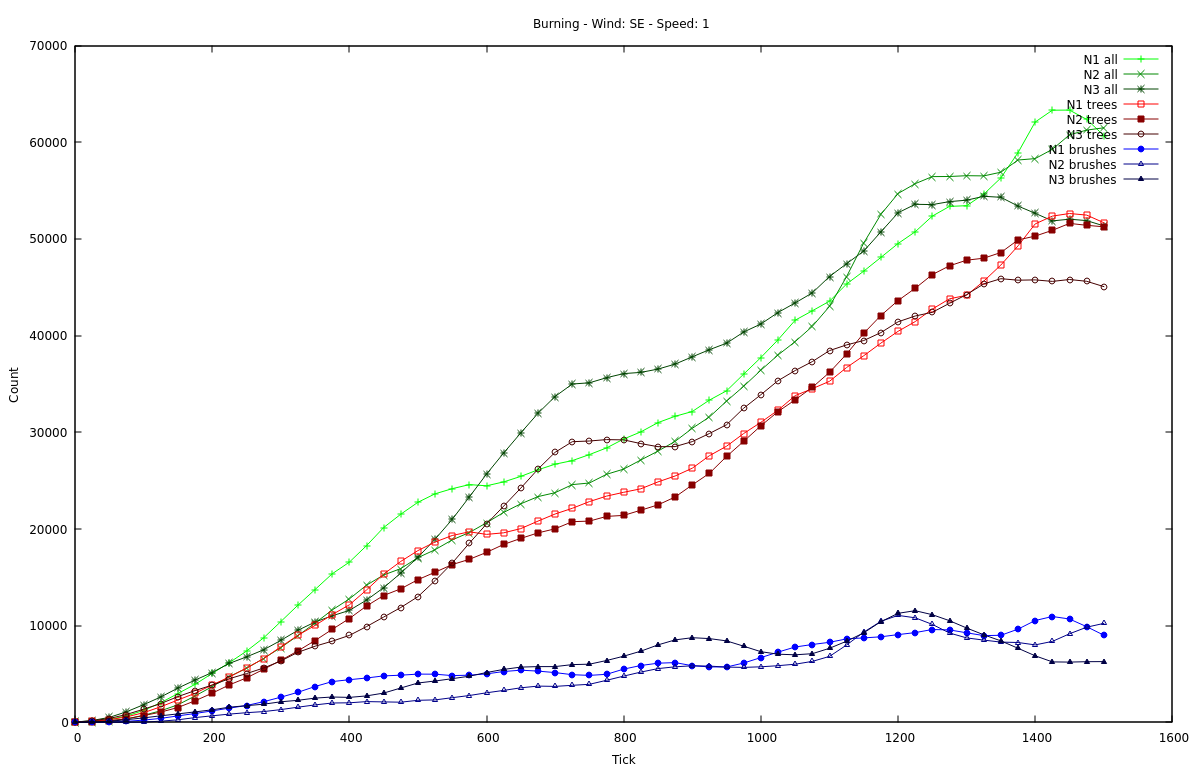
\includegraphics[width=8.2cm]{../output/burning/burning_se1.png} }}
    \subfloat[\centering Silný vietor]{{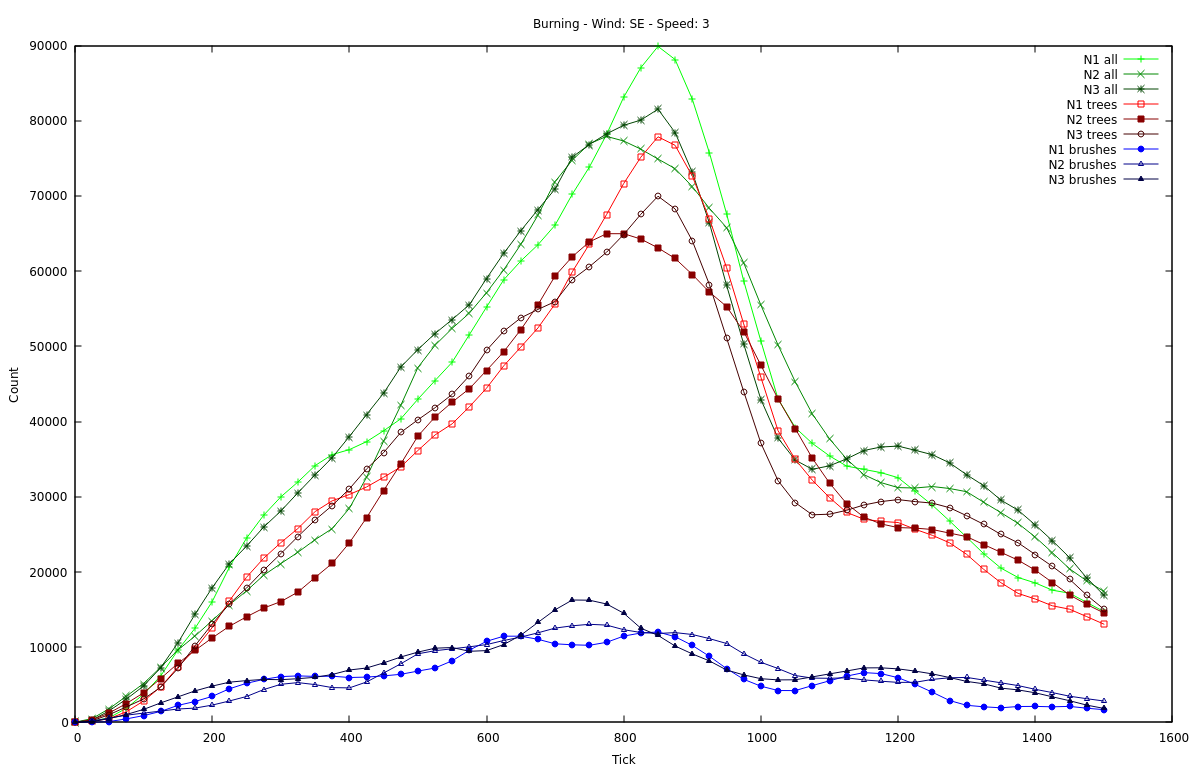
\includegraphics[width=8.2cm]{../output/burning/burning_se3.png} }}
    \caption{Grafy pre horiace bunky pri rôznych poveternostných podmienkach}

    \label{fig:burning}
\end{figure}

\FloatBarrier
\begin{figure}%
    \centering
    \subfloat[\centering Bezvetrie]{{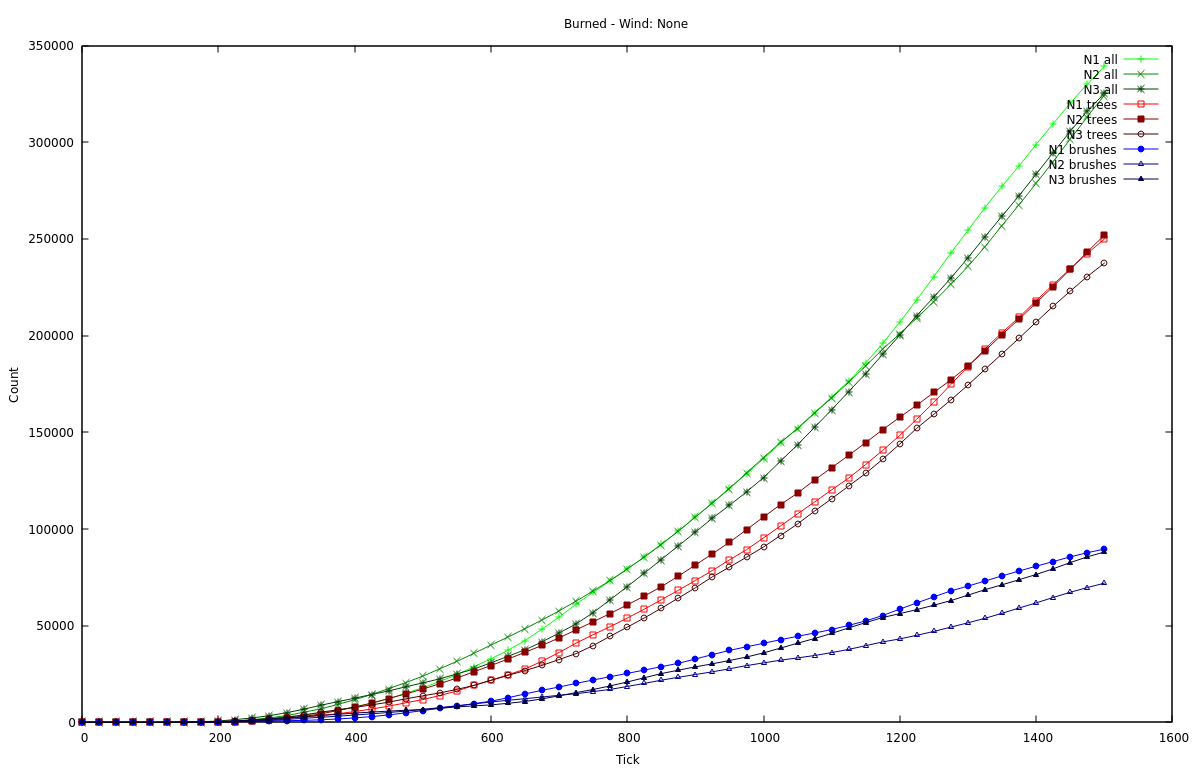
\includegraphics[width=8.2cm]{../output/burned/burned_none.png} }}
    \qquad
    \subfloat[\centering Slabý vietor]{{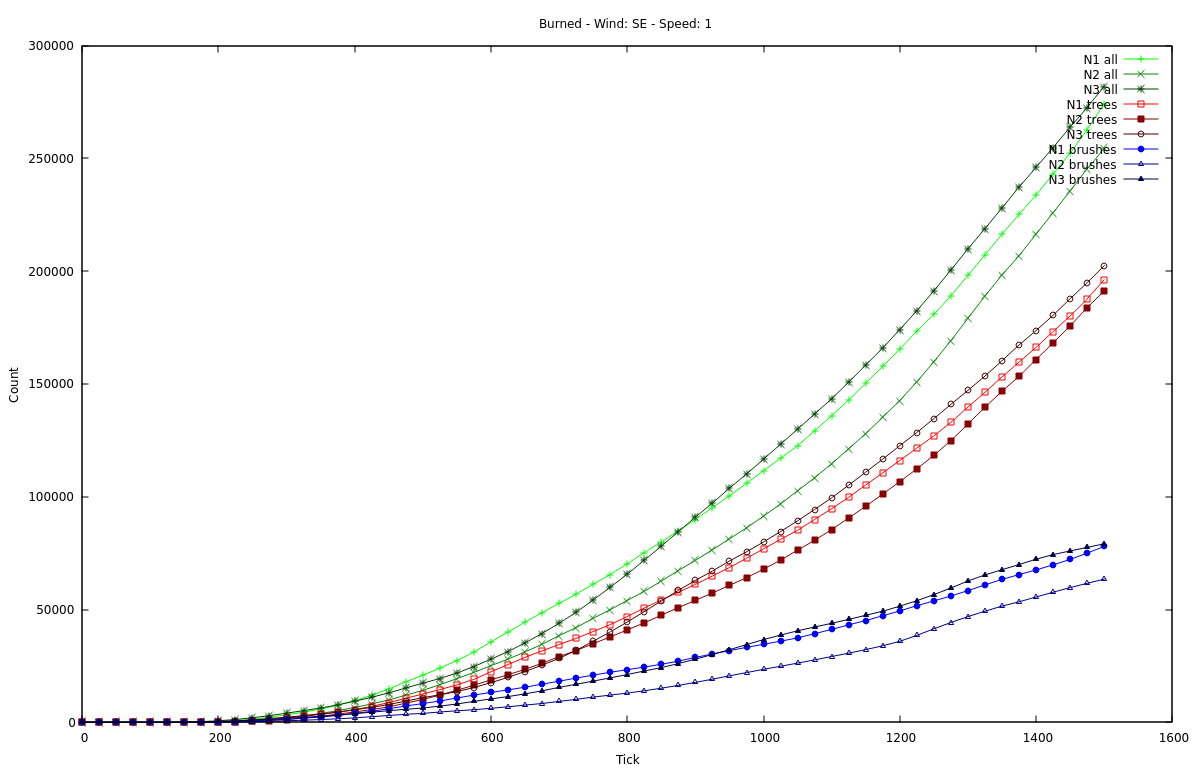
\includegraphics[width=8.2cm]{../output/burned/burned_se1.png} }}
    \subfloat[\centering Silný vietor]{{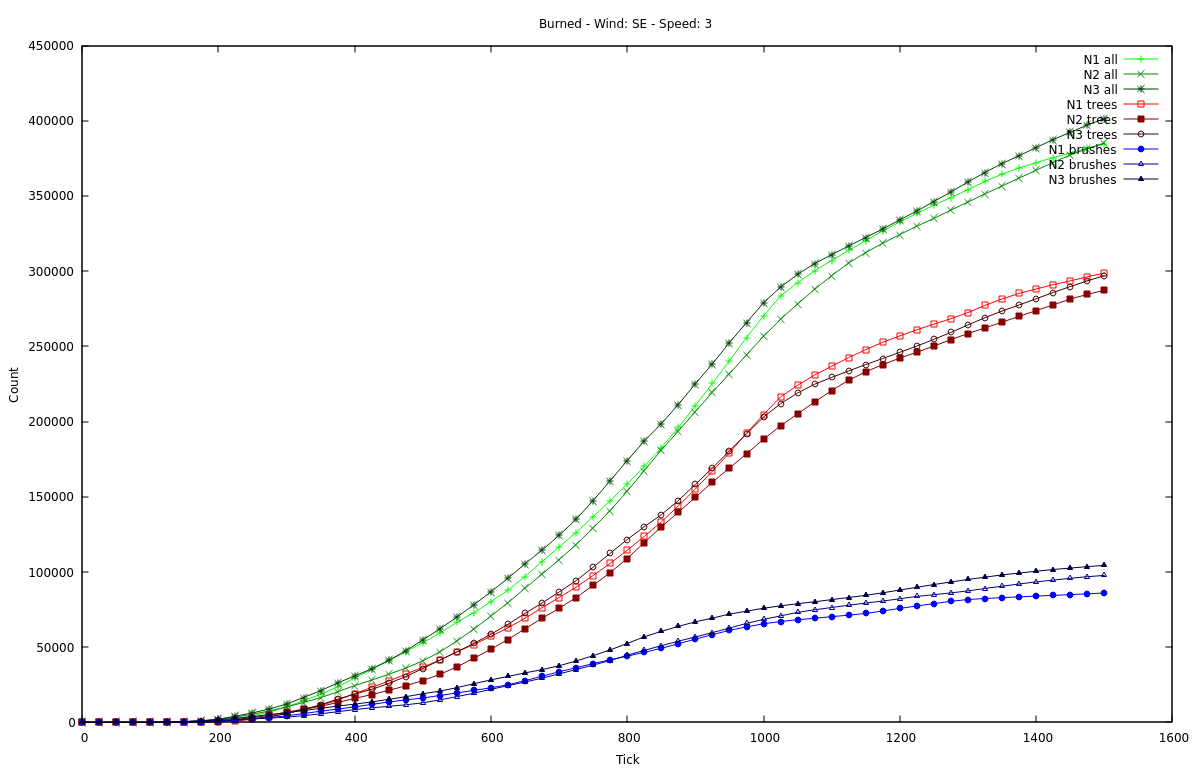
\includegraphics[width=8.2cm]{../output/burned/burned_se3.png} }}
    \caption{Grafy pre zhorené bunky pri rôznych poveternostných podmienkach}

    \label{fig:burned}
\end{figure}

\FloatBarrier
\begin{figure}%
    \centering
    \subfloat[\centering Bezvetrie]{{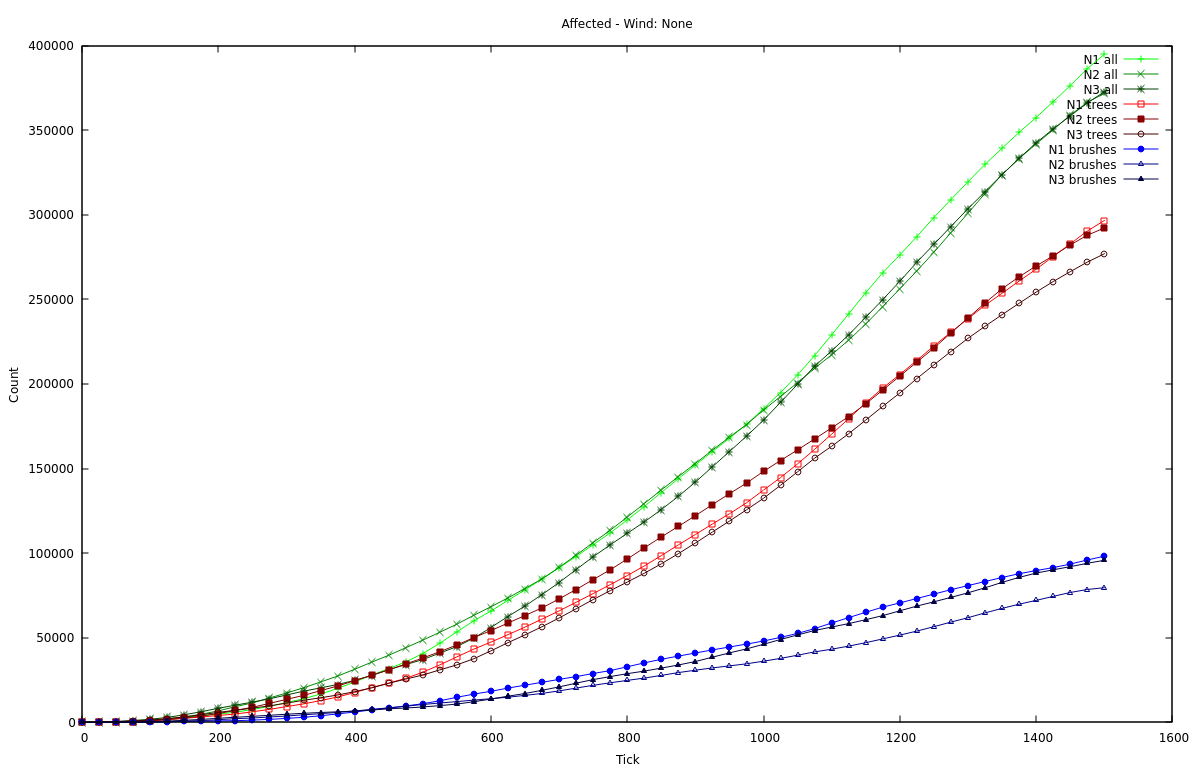
\includegraphics[width=8.2cm]{../output/affected/affected_none.png} }}
    \qquad
    \subfloat[\centering Slabý vietor]{{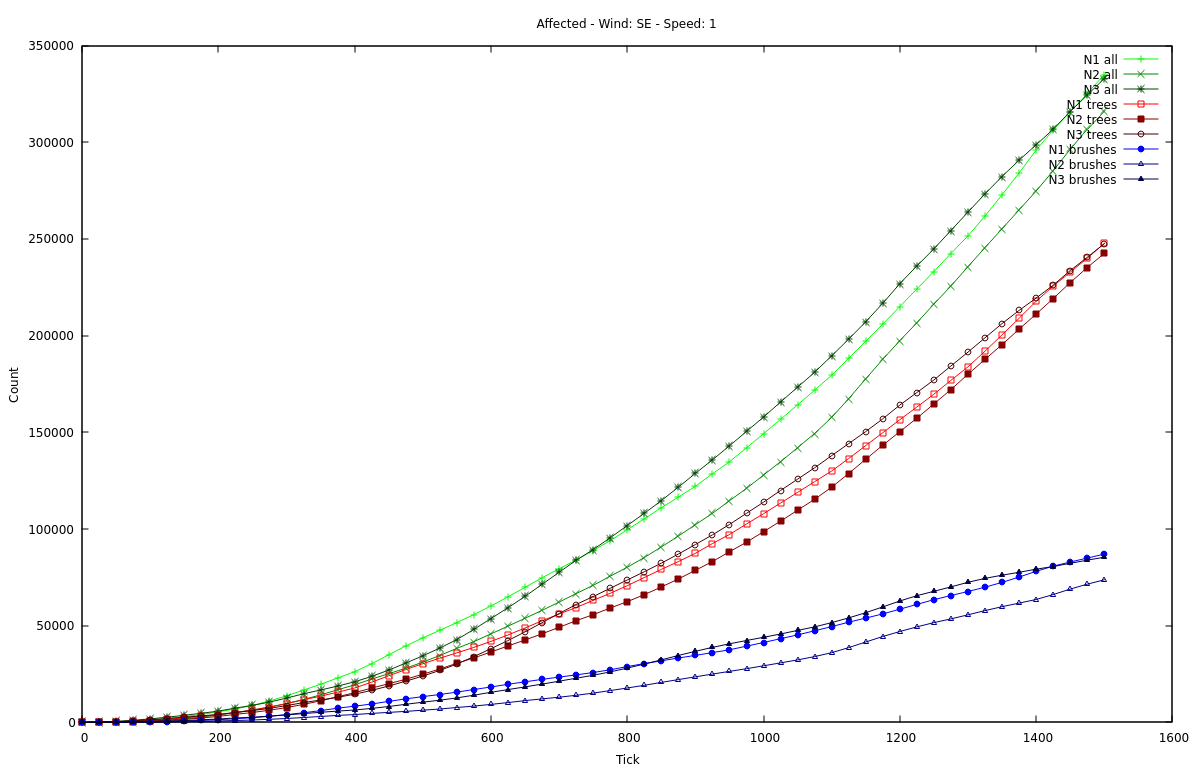
\includegraphics[width=8.2cm]{../output/affected/affected_se1.png} }}
    \subfloat[\centering Silný vietor]{{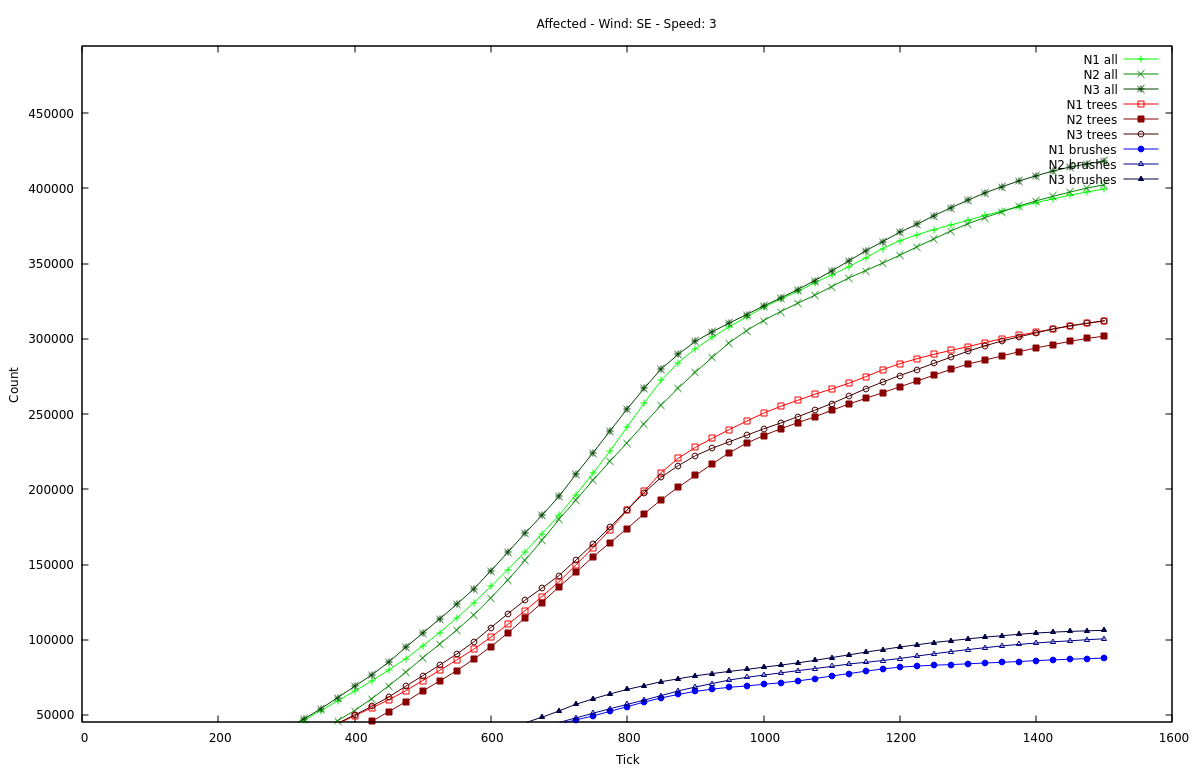
\includegraphics[width=8.2cm]{../output/affected/affected_se3.png} }}
    \caption{Grafy pre postihnuté bunky pri rôznych poveternostných podmienkach}

    \label{fig:affected}
\end{figure}
\FloatBarrier

\newpage
\section{Bibliografia}
\bibliographystyle{czechiso}
\bibliography{manual}
\nocite{CAmodel4FF}
\nocite{Pnoise}
\nocite{simulations}
\nocite{fireSpread}
\nocite{konceptModel}


\end{document}
